% !TeX root = ../artigo.tex
\section{GERADOR DE TRÁFEGO HTTP}

O protocolo HTTP, definido nos RFCs 1945 e 2616 é implementado em dois programas: cliente e servidor.

A interação entre estes programas, que estão sendo executados em diferentes dispositivos da rede ocorre por meio da troca de mensagens HTTP. Estas mensagens tem uma estrutura estabelecida e permitem a requisição, por parte do cliente, de recursos hospedados no servidor, conforme tratado na Figura \ref{fig:http-process}.

Quando um usuário solicita um recurso em um servidor web, este recurso pode ser identificado por uma URL (\textit{Uniform Resource Location}). Em outras palavras, o cliente envia uma mensagem de requisição ao servidor com indicando, por meio de uma URL, qual recurso deseja receber.

O servidor por sua vez, responde essa solicitação com uma mensagem de resposta e o recurso solicitado, quando este é localizado, é claro. Tais mensagens de requisição e repostas são padronizadas pelos RFCs 1945, 2616 e 7540 e formam o cabeçalho HTTP \cite{Kurose2013}.

Este cabeçalho HTTP poderia ser abstraído em uma implementação de gerador de tráfego HTTP para ambientes de simulação. Contudo, considerando que a presente proposta também tem como objetivo fomentar o estudo do protocolo, procedeu-se a implementação de uma versão simplificada deste cabeçalho.


\subsection{CABEÇALHO HTTP}

O trecho abaixo ilustra uma mensagem HTTP de requisição típica (adaptado de \cite{Kurose2013}). 

\begin{verbatim}
	GET /umaurl/algumrecurso.html HTTP/1.1
	Host: www.algumsite.com
	Connection: close
	User-agent: Mozilla/5.0
\end{verbatim}

A primeira linha desta mensagem é denominada linha de requisição (\textit{request line}). As linhas seguintes são as linhas de cabeçalho. 

Na linha de requisição podemos identificar três campos: o método (GET, POST, PUT), a URL e a versão do HTTP. Já as linhas de cabeçalho são formadas pelo nome do campo, acrescido de dois pontos (:), espaço e o valor para aquele campo.

A mensagem de requisição do cabeçalho HTTP implementada no módulo gerador proposto, por ora, apresenta apenas a linha de requisição. Essa simplificação atende as demandas do gerador de tráfego, enquanto abre espaço para futuras melhorias.

Para a mensagem de resposta, o trecho abaixo ilustra uma situação comum (adaptado de \cite{Kurose2013}):

\begin{verbatim}
	HTTP/1.1 200 OK
	Connection: close
	Date: Sun, 12 Dec 2021 22:18:05 GMT
	Server: Apache/2.2.3 (CentOS)
	Last-Modified: Fri, 10 Dec 2021 15:11:03 GMT
	Content-Length: 6821
	Content-Type: text/html
	
	(data data data data ...)
\end{verbatim}

A estrutura da mensagem de reposta é composta por três partes: linha de estado (\textit{status line}), linhas de cabeçalho e corpo da entidade.

A linha de estado apresenta a versão do HTTP, o código de estado do recurso e a frase de estado correspondente. As linhas de cabeçalho apresentam informações sobre a conexão, servidor e detalhes do recurso solicitado. Por fim, o corpo da entidade traz o recurso propriamente dito.

A mensagem de resposta implementada no gerador de tráfego proposto apresenta a linha de estado, o corpo da entidade e possibilita o uso de quantas linhas de cabeçalho a aplicação servidora desejar enviar ao cliente.

\subsubsection{Implementação no ns-3}
O ns-3 apresenta uma estrutura de diretórios com organização pré-definida. Os cabeçalhos de protocolos se encontram no diretório \verb|src/internet/|. Escrito em C++, o código de implementação apresenta as estruturas necessárias para a montagem do cabeçalho por parte da aplicação definidos em arquivos com extensão \verb|.h| e \verb|.cc|.

Por ser um projeto de grande escala, desenvolvido por pesquisadores e desenvolvedores do mundo inteiro, o consórcio que gerencia o desenvolvimento do simulador estabeleceu regras para a escrita do código, conforme apresentado em \cite{ns-3-contributing}. Neste sentido, o ns-3 utiliza o Doxygen como ferramenta para gerar a documentação a partir dos comentários inseridos ao longo do código fonte. A Figura \ref{fig:doxygen-comments} apresenta um trecho de código de um gerador de tráfego já presente no ns-3. Repare que antes da declaração do construtor da classe, existe um comentário explicativo. Na Figura \ref{fig:api-documentation} tem-se um trecho da documentação da API do ns-3 gerada com o Doxygen a partir dos comentários inseridos no código fonte e disponibilizada na web \cite{ns-3-api}.


\begin{figure}
	\centering
	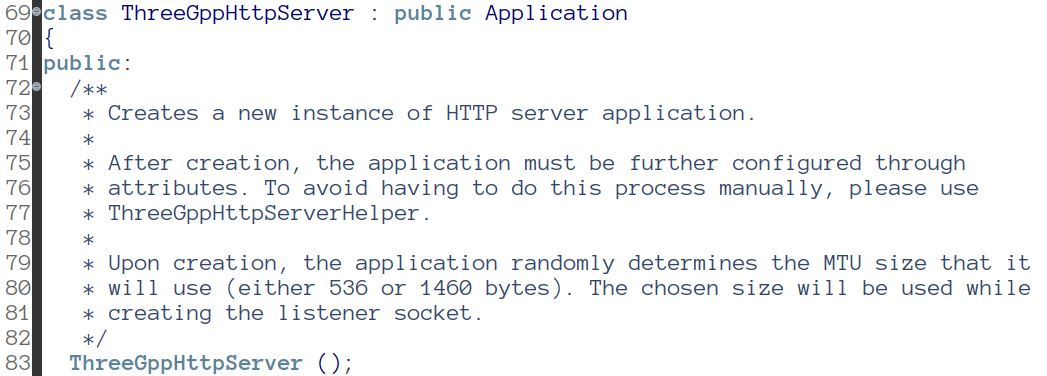
\includegraphics[scale=0.5]{textuais/doxygen-comments.jpg}
	\caption[Comentários no código fonte.]{Comentários no código fonte.).
		\label{fig:doxygen-comments}}
\end{figure}


\begin{figure}
	\centering
	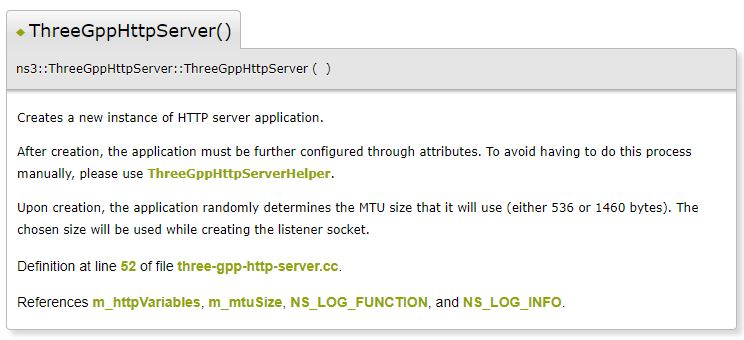
\includegraphics[scale=0.75]{textuais/api-documentation.jpg}
	\caption[Documentação da API da classe gerada via doxygen]{Documentação da API da classe gerada via doxygen.
		\label{fig:api-documentation}}
\end{figure}

Para o cabeçalho HTTP desenvolvido no projeto, seguiu-se a mesma estratégia, conforme ilustrado na Figura \ref{fig:header-comments}. 

\begin{figure}
	\centering
	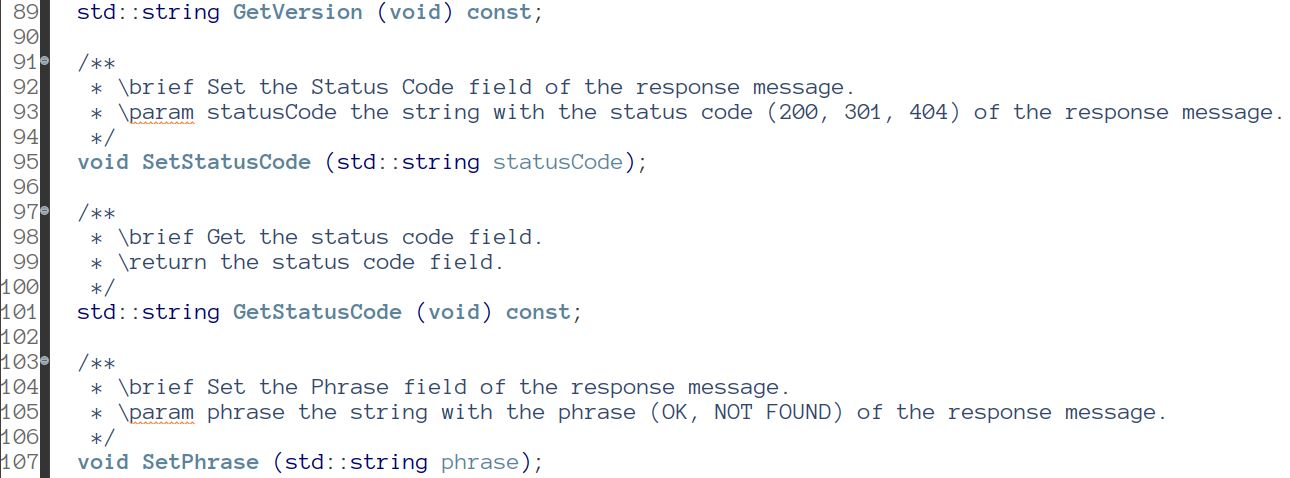
\includegraphics[scale=0.45]{textuais/header-comments.jpg}
	\caption[Comentários no código do cabeçalho para futura documentação.]{Comentários no código do cabeçalho para futura documentação.
		\label{fig:header-comments}}
\end{figure}

Outro aspecto importante da implementação é a abordagem realista estabelecida pelo ns-3 para o cabeçalho. Os valores dos campos do cabeçalho são "serializados" e "deserializados" no processo de implementação do código conforme ilustrado na Figura \ref{fig:serialize-deserialize}. Esse mecanismo resulta em um cabeçalho que pode ser registrado em arquivos de captura de pacotes de rede, como por exemplo o tradicional formato \verb|.pcap|. Ao serem lidos por uma aplicação adequada como o Wireshark, estes arquivos \verb|.pcap| revelam a estratégia realista da implementação. A Figura \ref{fig:pcap-real-simulado} apresenta duas capturas: uma realizada via simulação no ns-3 e a outra em uma rede real. É possível observar que a implementação do cabeçalho está em consonância com os requisitos estabelecidos pelo ns-3 e organizações de padronização para redes reais. A implementação da mensagem de requisição no cabeçalho proposto apresenta apenas a linha de requisição. Contudo, novas versões poderão apresentar os outros campos e possibilitar novas análises.

\begin{figure}[h]
	\centering
	\begin{subfigure}[t]{\textwidth}
		\centering
		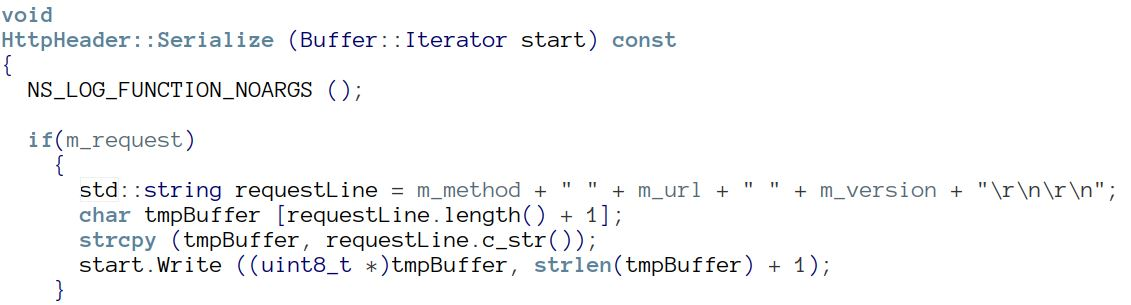
\includegraphics[width=0.9\linewidth]{textuais/serialize.jpg}
		\caption{Serialização.}
		%\label{fig:sub1}
	\end{subfigure}
	\begin{subfigure}[t]{\textwidth}
		\centering
		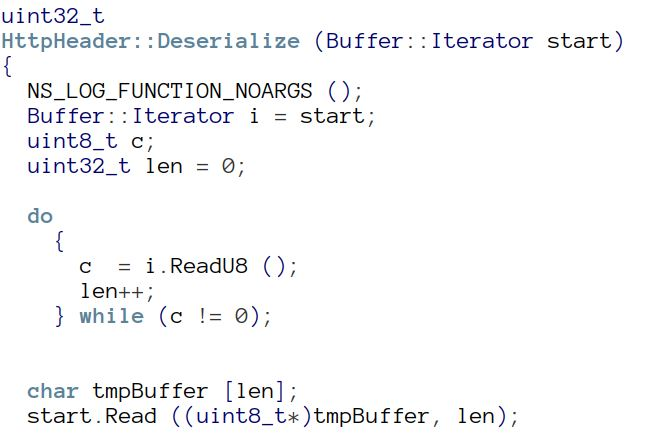
\includegraphics[width=0.5\linewidth]{textuais/deserialize.jpg}
		\caption{Deserialização.}
		%\label{fig:sub2}
	\end{subfigure}
	\caption{Métodos de serialização e deserialização.}
	\label{fig:serialize-deserialize}
\end{figure}


\begin{figure}[h]
	\centering
	\begin{subfigure}{\textwidth}
		\centering
		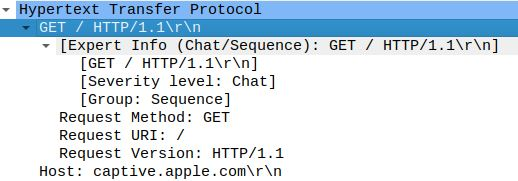
\includegraphics[width=0.6\linewidth]{textuais/pcap-real-capture.jpg}
		\caption{Cabeçalho HTTP real.}
		%\label{fig:sub1}
	\end{subfigure}
	\begin{subfigure}{\textwidth}
		\centering
		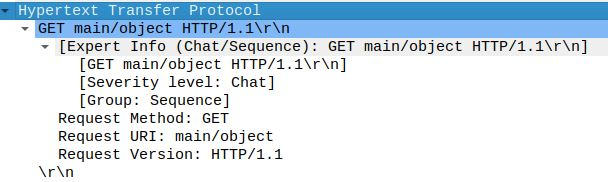
\includegraphics[width=0.6\linewidth]{textuais/pcap-simulated-capture.jpg}
		\caption{Cabeçalho HTTP simulado.}
		%\label{fig:sub2}
	\end{subfigure}
	\caption{Comparação de capturas de pacotes em rede real e simulada.}
	\label{fig:pcap-real-simulado}
\end{figure}

\subsection{APLICAÇÕES CLIENTE E SERVIDOR}

O cabeçalho HTTP fomenta maiores estudos em torno do funcionamento do protocolo HTTP. Contudo, o núcleo principal do gerador de tráfego proposto são as aplicações cliente e servidor.

No ns-3, as aplicações estão localizadas no diretório \verb|/src/applications/|. Dentro deste diretório é possível identificar algumas outras pastas. Dentre elas podemos destacar \verb|model|, \verb|helper| e \verb|examples|.

No diretório \verb|model| encontram-se as implementações dos modelos das aplicações do ns-3. Já no diretório \verb|helper| estão programas auxiliares que facilitam o uso das aplicações nos scripts de simulação. Por fim, a pasta \verb|examples| apresenta exemplos de utilização das aplicações, que facilitam o uso por parte de novos usuários.

O gerador proposto segue o comportamento descrito anteriormente para aplicações baseadas no HTTP, isto é, um cliente solicita um dado recurso que está armazenado em um servidor remoto. O servidor por sua vez, encontra o recurso e envia para o cliente solicitante.

Do lado da aplicação cliente, o gerador de tráfego implementa uma aplicação simples. Ao receber, via script de simulação, as informações de endereço IP e porta de trabalho do servidor, o cliente cria um socket TCP e inicia o processo de estabelecimento da sessão TCP. Se o servidor está operante, este recebe o pedido de sessão e realiza os procedimentos do tradicional \textit{three-way handshake}. Aqui vale ressaltar as vantagens da implementação do gerador de tráfego dentro de um ambiente de simulação como o ns-3. Toda a pilha de protocolos já está estabelecida, facilitando o trabalho dos desenvolvedores das aplicações e dando maior realismo à simulação.

Com a sessão TCP estabelecida, o cliente envia, então, uma mensagem HTTP de requisição, passando a url \verb|main/object| e indicando que deseja receber o objeto principal de uma página web genérica. Em seguida, o cliente entra em modo de espera, aguardando o envio dos dados. Ao receber todos os dados, a aplicação cliente utiliza o modelo matemático apresentado em \cite{Pries2012} para calcular o tempo de leitura do usuário, antes de realizar uma nova solicitação por outro recurso no servidor. A Figura \ref{fig:http-client} ilustra esse fluxo de funcionamento.

\begin{figure}
	\centering
	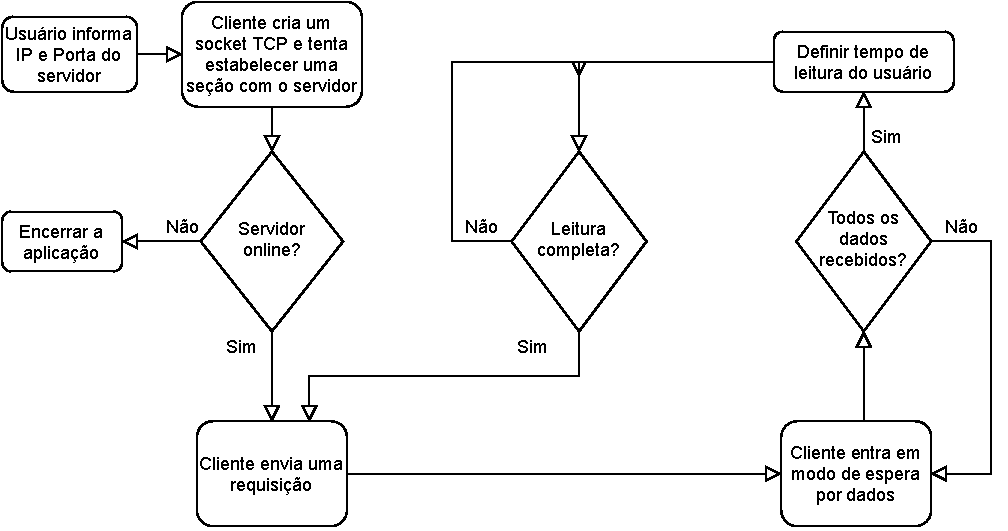
\includegraphics[scale=0.75]{textuais/http-client.pdf}
	\caption[Fluxograma do funcionamento do cliente HTTP.]{Fluxograma do funcionamento do cliente HTTP.
		\label{fig:http-client}}
\end{figure}

Do lado da aplicação servidora, o programa recebe a porta de trabalho via script de simulação, inicia um socket TCP e fica aguardando solicitações de criação de sessão.

Ao receber e aceitar uma sessão TCP, o servidor HTTP passa para o modo de espera por requisições web. Ao receber a requisição, a aplicação estabelece os parâmetros das respostas, tais como, tamanho do objeto principal, número e tamanho dos objetos \textit{inline}, com base no modelo matemático apresentado em \cite{Pries2012}. Assim que todos os dados solicitados são entregues, o servidor volta ao modo de espera por novas requisições. A Figura \ref{fig:http-server} ilustra esse processo. 

\begin{figure}
	\centering
	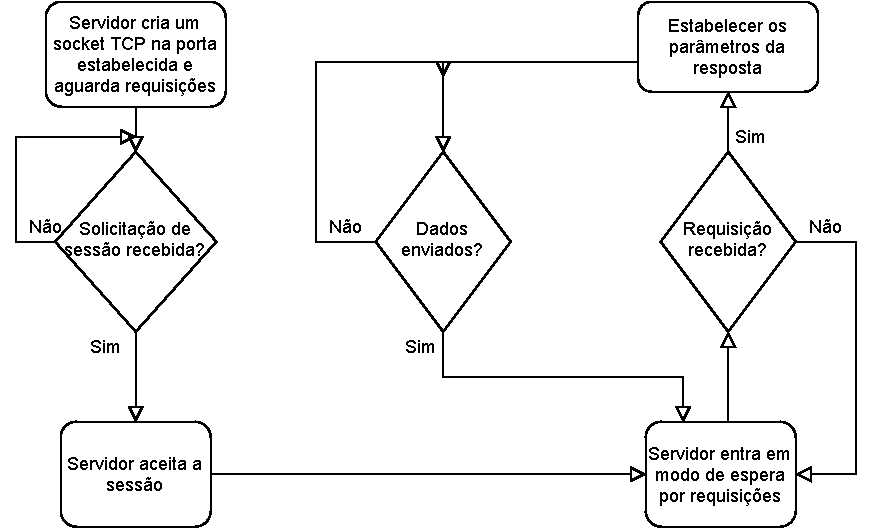
\includegraphics[scale=0.75]{textuais/http-server.pdf}
	\caption[Fluxograma do funcionamento do servidor HTTP.]{Fluxograma do funcionamento do servidor HTTP.
		\label{fig:http-server}}
\end{figure}

